\documentclass[conference]{IEEEtran}
\IEEEoverridecommandlockouts
% The preceding line is only needed to identify funding in the first footnote. If that is unneeded, please comment it out.
\usepackage{cite}
\usepackage{amsmath,amssymb,amsfonts}
\usepackage{algorithmic}
\usepackage{graphicx}
\usepackage{textcomp}
\usepackage{xcolor}
\def\BibTeX{{\rm B\kern-.05em{\sc i\kern-.025em b}\kern-.08em
    T\kern-.1667em\lower.7ex\hbox{E}\kern-.125emX}}

\begin{document}


%
% paper title
% Titles are generally capitalized except for words such as a, an, and, as,
% at, but, by, for, in, nor, of, on, or, the, to and up, which are usually
% not capitalized unless they are the first or last word of the title.
% Linebreaks \\ can be used within to get better formatting as desired.
% Do not put math or special symbols in the title.
\title{ Machine Translation}


% author names and affiliations
% use a multiple column layout for up to three different
% affiliations
\author{
    \IEEEauthorblockN{Rayforth Brenes Rodríguez}
    \IEEEauthorblockA{rayforth1616@estudiantec.cr}
    \and
    \IEEEauthorblockN{Jesús Cortés Álvarez}
    \IEEEauthorblockA{cortesj02@estudiantec.cr}
    \and
     \IEEEauthorblockN{Andrew López Herrera}
    \IEEEauthorblockA{andrewlopezherrera@estudiantec.cr}
    \and
     \IEEEauthorblockN{Alex Sánchez Céspedes}
    \IEEEauthorblockA{alex27@estudiantec.cr}
}


% make the title area
\maketitle

% As a general rule, do not put math, special symbols or citations
% in the abstract
\begin{abstract}
La brecha creada por las diferencias en los idiomas existentes en el mundo han dificultado distintos campos en la sociedad como la política y la economía. Como posible solución a estos problemas ha aparecido la traducción automática.
Esta nueva tecnología intenta traducir texto de un idioma a otro, sin la intervención humana. En este documento se presentará un poco sobre la historia del MT (Machine Translation) y los principales métodos de traducción automática.

\end{abstract}

\IEEEpeerreviewmaketitle

\section{Introducción}

A lo largo del tiempo, la comunicación en el sector económico, político y cultural ha sido uno de los temas de más importancia para un buen desarrollo integral de una sociedad, pero este desarrollo se ve afectado por las barreras lingüísticas que generan las distintas lenguas y dialectos existentes en el mundo, adicionando que el proceso para traducir dicha información se realizaba de manera manual, lo cual requería de mucho tiempo, recursos y habilidades especializadas.

Esta situación impulsó el desarrollo de las máquinas traductoras, que con el paso del tiempo se han convertido en una herramienta fundamental, facilitando la comunicación entre las personas de diferentes países.

El enfoque principal de estas máquinas es la de ayudar en la tarea de la traducción del contenido de un idioma a otro sin la intervención humana, esta idea nace en el año 1950, cuando los científicos intentaron usar la potencia de cálculo de los ordenadores de ese tiempo para automatizar la traducción de texto, sin embargo, descubrieron que la complejidad de esta tarea era muy superior al potencial de los ordenadores y se desecharon todos los incentivos sobre la investigación y desarrollo de estas máquinas.

Esto ejemplifica que el proceso de manipulación y traducción de ideas de un texto en un idioma específico es un trabajo de suma complejidad debido a la diferencia que pueda existir entre los lenguajes, esto teniendo en cuenta que las ideas expresadas en un lenguaje puede tener varias formas diferentes en las que se puede expresar en otro idioma.

Sin embargo, en los últimos años los avances en el software y hardware han hecho posible la traducción automática, gracias a un previo y constante entrenamiento de estas máquinas se logró realizar las primeras traducciones básicas de un idioma a otro, no obstante, este proceso de aprendizaje consumía mucho tiempo y estas máquinas debían reiniciar el proceso por cada idioma distinto.
\vspace{2.0cm}
Con esto nacen distintos métodos de traducción con la intención de facilitar aún más el proceso, estos métodos se conocen como:

\begin{itemize}
    \item MT basada en reglas
    \item MT estadística
    \item MT basada en ejemplos
    \item MT neuronal
\end{itemize}

Cada una presenta diferencias en su funcionamiento y algunas son más recomendables y eficientes que otras, toda la información sobre estas se detallaran en otra sección.

Por otro lado, la traducción automática moderna presenta una serie de errores en sus resultados, algunos de estos problemas pueden surgir a partir de problemas gramaticales, malentendidos culturales e inconsistencias terminológicas, y esto afecta negativamente la calidad de la traducción.

Existen algunos problemas ya conocidos en la traducción automática moderna, por ejemplo:

\begin{itemize}
    \item Errores léxicos
    \item Errores sintácticos
    \item Errores semánticos
    \item Errores orto tipográficos
    \item Errores de contexto
\end{itemize}


Estos errores nos reflejan que aún es necesario mejorar los métodos de traducción automática, si lo que se busca es la mayor eficiencia en este proceso, todos estos errores serán detallados en secciones posteriores.

\section{Desarrollo}
\subsection*{Definición de MT (Machine translation)}

La traducción a diferentes idiomas, según el que sea necesario, ha sido una acción recurrente en las diferentes etapas de la vida humana, como consultoría o como aprendizaje, el término ya era usado o pensado desde el siglo XVII, pero siglos después ese pensamiento se comenzó a materializar y año tras año ha mejorado gracias a las grandes mentes detrás de la traducción automática (TA) o en inglés Machine Translation (MT).

La siguiente persona autora menciona en qué consiste la traducción automática:
” Machine translation is not primarily an area of abstract intellectual inquiry but the application of computer and language sciences to the development of systems answering practical needs.”\cite{b3}

El autor John Hutchins menciona la forma en que las ciencias informáticas y del lenguaje en el desarrollo de sistemas responde a necesidades prácticas, en otras palabras, lo anterior menciona como la traducción automática no posee intervención humana, sino mediante programas de computadora. Viéndolo de esa forma, parece ser un procedimiento que podría resultar fácil y sin mucha dificultad, que podría funcionar con un simple clic.

Sin embargo, no es de esa forma, la parte computacional detrás en la fabricación de un traductor automático está compuesta por gran variedad de conceptos como algoritmos, diccionarios y demás fuentes de información. Este sistema es de suma importancia, sea para el ámbito en el que sea utilizado como grandes empresas, como procesos de comunicación, recepción de textos, como también en diccionarios en línea.

Anteriormente, se comentó, como para el desarrollo de los programas de traducción automática se necesita gran cantidad de información como, vocabulario, gramática, estructuras de oraciones más complejas, las cuales siempre son necesarios para mejorar la calidad del programa, no obstante, por más compleja que sea la programación, no siempre presenta exactitud en las traducciones, el autor John Hutchins explica que es probable que se presenten problemas de ambigüedad y se utilicen traductores para poder resolver los problemas que en ciertos casos puedan ocurrir durante el proceso de traducción. \cite{b3}

Al utilizar un sistema como este y aspectos como que es necesario la intervención humana en algunos casos, ejemplifica que la utilización de la traducción automática, remplazaría a los traductores humanos o ya no sería necesaria su aporte en diferentes entidades que requieran traducciones para las actividades que la requieran, esto por el temor causado por los grandes avances de la tecnología, al utilizarla actualmente en diferentes ámbitos.

“Así mismo, como puede ser de suma importancia para grandes corporaciones para diferentes tareas, la traducción automática puede ser de gran ayuda para el aprendizaje y con base en esto, como lo hacen notar (Grace, Paul, 2009): “MT can be efficiently applied as a superior way of teaching and learning…such as translating a textbook or teaching and learning a course, and what types of software can be successfully applied.”\cite{b5}

Haciendo énfasis se logra visualizar como las MT pueden ser una herramienta muy importante para el aprendizaje, como por ejemplo en libros de texto.

Al inicio, cuando se definía la traducción automática, se mencionaba que desde hace más de tres siglos se tenía en mente la traducción de lenguaje natural realizado por una máquina. A lo largo de historia ha habido avances de los cuales la traducción automática fue de gran ayuda, historias como lo fueron guerras, avances en el aprendizaje, facilitar el trabajo para empresas a nivel mundial, todo esto debido a la necesidad de comunicación entre clientes, así también como para crear relaciones entre países.

La implementación de la traducción y sus primeras implementaciones a inicios de los años treinta por George Arstsrouni y por Petr Smirnov Troyanskii, el primero realizó una cinta de papel, la cual almacenaba y se usaba para encontrar el equivalente de una palabra a otro idioma.

\vspace{1.6cm}
Según el autor, Troyanskii planteó lo siguiente:

"First, an editor knowing only the source language was to undertake the 'logical' analysis of words into their base forms and syntactic functions; secondly, the machine was to transform sequences of base forms and functions into equivalent sequences in the target language; finally, another editor knowing only the target language was to convert this output into the normal forms of his own language".\cite{b3} sale troyanskii

Troyanskii desarrolló esta traducción automática de forma que imaginó una traducción bilingüe y multilingüe, además gracias al análisis lógico que creó, pensó que era posible mecanizarse lo que había planteado. Pero años después Warren Weaver y Andrew D.Booth propusieron la idea de utilizar la computación para la traducción. Continuamente en Cambridge, Richard H.Richens realizaba traducciones palabra por palabra mediante tarjetas perforadas para resúmenes científicos.

“Fue hasta 1954 que se proyectó por primera vez un sistema MT, realizado por la Universidad de Georgetown junto a la colaboración de IBM, dicho sistema realizó cuidadosamente una traducción al inglés de 49 oraciones rusas, usando poco vocabulario y tres reglas gramaticales”. \cite{b3}.%revisar cita, no es la dos, es hutchins, no sale

Este hecho creó grandes expectativas, ya que en un futuro muy cercano se podrían desarrollar sistemas de traducción automática capaces de realizar traducciones de mucha más alta calidad.

“Contando unos 7.700 millones de habitantes en el planeta, Google Translate procesa unas 20
palabras por persona al día. Se puede argumentar que este cálculo no es indicativo de
cuántas de estas palabras traducidas se usan. Es posible que un usuario traduzca una
web aprovechando la extensión de Google Translate del navegador, pero únicamente
esté interesado en conocer el significado de tres o cuatro palabras.”\cite{b13}


\subsection{Tipos y algoritmos utilizados en el MT (Machine translation)}
En la actualidad, existen varios tipos o formas en las que se realiza el proceso de traducción automática, los cuales varían en su enfoque y en la calidad de los resultados, estos tipos son:

\subsection{MT basado en reglas}

Los métodos basados en reglas parten de las herramientas o recursos lingüísticos para crear una traducción. Se basan en reglas lingüísticas y gramaticales del idioma, así como en diccionarios con palabras comunes del idioma, por lo cual se requieren extensos léxicos con información morfológica, sintáctica, semántica, y grandes conjuntos de reglas.
Estas reglas se utilizan para luego transferir la estructura gramatical del idioma de origen al idioma de destino.\cite{b2}

Como menciona Borges, este tipo de traducción automática emplea reglas sintácticas y morfológicas para realizar la traducción de la información, estos sistemas vinculan una frase de entrada con otra frase del lenguaje destino como salida, lo que ayuda a mantener el sentido o significado del texto.

En la Figura 1 podemos observar un modelo simple del funcionamiento de este tipo de traducción.

\begin{figure}[htp]
        \centering
        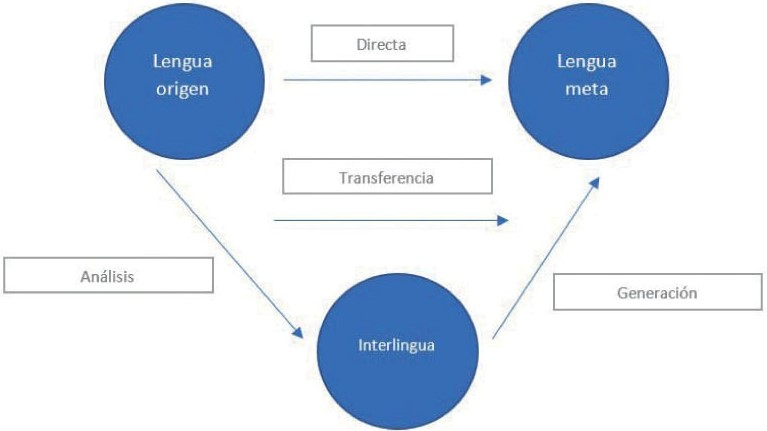
\includegraphics[width=8cm]{MT basado en reglas.jpeg}
        \label{foto}
        \caption{Descripción gráfica del funcionamiento de un motor de TA basado en reglas}
    \end{figure}
\vspace{3cm}

Algunos de los requisitos para realizar una traducción de este tipo tenemos:
\begin{itemize}
    \item Un diccionario que asocie las frases o palabras del idioma original al idioma destino.
    \item Reglas de estructuración de cada idioma, tanto gramaticales como sintácticas.
\end{itemize}

Este tipo de TA se caracteriza por requerir de una gran inversión de tiempo y recursos, ya que es necesario contar con la información sobre la gramática del idioma origen y del idioma destino, así como también diccionarios.

“Otra desventaja de este método es que no puede traducir estructuras lingüísticas que no estén en la gramática del modelo o en sus reglas de transferencias, tampoco puede reconocer palabras que no se encuentren en sus diccionarios. Por lo tanto, el mantenimiento de estos métodos debe ser casi continuo para asegurar que traduzcan textos nuevos o estructuras que no estén previstas.”\cite{b2}

Una ventaja de este tipo de TA es cuando se desea traducir idiomas con un corpus sencillo o pequeño, lo cual facilita el proceso de traducción y recorta el tiempo y recursos necesarios para el proceso. 

Actualmente, existen algunos TA basados en reglas como:
\begin{itemize}
    \item Apertium
    \item Systran
    \item SDL MultiTerm
\end{itemize}


\subsection{MT basado en ejemplos}
No fue hasta la década de 1980 que las computadoras obtuvieron una evolución en cuanto a la capacidad de almacenamiento de datos, lo que genero la disponibilidad de bases de datos más grandes, abriendo la posibilidad de aprovecharlas de manera sistemática para la traducción automática.

Fue en este contexto que surgió la idea de la MT basada en ejemplos, que se propuso por primera vez en Japón en 1984. Estos sistemas se basaron en el análisis de los patrones que se encuentran en los textos de origen y destino para generar traducciones más precisas y naturales.

Asimismo, los sistemas basados en ejemplos utilizan bases de datos de ejemplos conocidos para generar nuevas traducciones, aquí se proporciona al sistema un conjunto de frases en el idioma origen y luego también se le proporciona las traducciones correspondientes en el idioma destino.
Dichas traducciones se realizan mediante la sustitución de frases que se identificaron como equitativas.

	Sin embargo, este tipo de traducción tiene sus limitaciones, ya que solo funciona con frases similares a las que se han usado en un pasado, además de necesitar una gran cantidad de texto bilingües paralelos para garantizar una eficiencia promedio en las traducciones.
	
En resumen, la MT basado en ejemplos fue una herramienta útil para ciertos contextos, pero ha sido superada por la MT estadística y la MT neuronal en términos de precisión y la capacidad de manejar o procesar una amplia variedad de idiomas y estructuras gramaticales. 
\begin{figure}[htp]
        \centering
        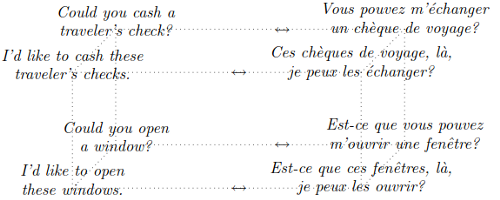
\includegraphics[width=9cm]{mt basado en ejemplos.png}
        \label{foto}
        \caption{Demostración de frases en idioma Inglés con su respectiva frase equivalente en idioma Frances.}
    \end{figure}



\subsection{Machine translation estadística}
Como su nombre lo dice, el Machine Translation estadístico trata de hacer las traducciones con base a métodos estadísticos utilizando textos bilingües. este MT no utiliza reglas gramaticales para traducir los textos, sino que depende de grandes cantidades de textos ya traducidos, estos textos son los que ya han sido traducidos por humanos, esto funciona detectando los patrones en esos textos ya traducidos.

Este MT funcionaba alimentando al software de una serie de textos ya traducidos, para que el sistema hiciera un análisis estadístico y produjera un texto de inglés a español, por ejemplo, con una traducción derivada de los análisis estadísticos que hacía el sistema. El texto producido tenía muchos aciertos y muchos errores, después el traductor humano tenía que limpiar todas las fallas e implementar las correcciones necesarias.

\begin{figure}[htp]
        \centering
        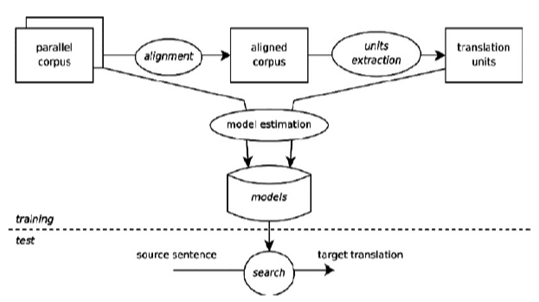
\includegraphics[width=8.5cm]{mt estadistico.png}
        \label{foto}
        \caption{Descripción gráfica de un sistema de traducción automática estadística.}
    \end{figure}


A pesar de este ser el método de traducción más utilizado últimamente, tiene sus ventajas y sus desventajas.
Las ventajas son que, este método de traducción es mejor que otros, ya que se basa en traducciones anteriores, es mejor en cuanto al rendimiento y los costos y es muy útil para prevenir los errores que se cometen cuando se presenta alguna excepción gramatical.

En cuanto a las desventajas, tenemos que el traductor no aprende de las correcciones del traductor humano, entonces va a seguir cometiendo los mismos errores una y otra vez, también que genera tarifas menores al traductor humano quien tenía que limpiar el texto porque las empresas o clientes piensan que el hecho de solo corregir errores es algo muy fácil entonces merecían una tarifa menor.

\subsection{Machine translation neuronal}
Esto es lo más nuevo que tenemos en el siglo XXI en cuanto a traducción automática, en este caso ahora si tenemos lo mejor de la inteligencia artificial combinado con la experiencia del traductor humano, ambos van a colaborar para producir la mejor traducción posible.

Entonces, si introducimos un texto a un software de traducción automática neuronal, vamos a tener de resultado lo mejor de dos mundos, ya que como dijimos anteriormente van a trabajar juntos la inteligencia artificial con el traductor humano, también vamos a obtener que el sistema aprenda, esto sería cuando el traductor humano le corrige sugerencias de traducción automática al software, el software se fija en eso y aprende gracias a la inteligencia artificial.

También vamos a tener que las tarifas para el traductor humano van a ser justas, ya que ahora colabora junto al software para crear la mejor traducción posible.

La traducción automática neuronal utiliza muchos más datos y menos algoritmos, esto da como resultado traducciones mucho más naturales.

“La traducción automática neuronal agrupa operaciones recurrentes que mapean un fragmento, palabra o conjunto de palabras en relación con las palabras con las que se integran, lemas que, a su vez, son mapeados de modo similar.”\cite{b13}

\begin{figure}[htp]
        \centering
        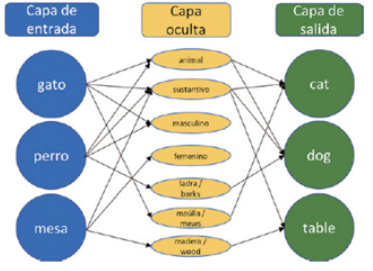
\includegraphics[width=8.5cm]{mt neural.png}
        \label{foto}
        \caption{Funcionamiento red neuronal artificial}
    \end{figure}
\vspace{2cm}
\subsubsection*{Ventajas}
\begin{itemize}
    \item Mucha más productividad
    \item Presenta buena estructura gramatical
    \item Reducción de errores: Para este punto compararemos el sistema E2E contra el sistema en cadenas. Los sistemas en cadena tienen la desventaja de acumular los errores que se generan por los módulos de la cadena. “Estos errores se propagan en la cadena de procesamiento global debido a la independencia de los módulos de tratamiento de los distintos aspectos (reconocimiento, traducción o síntesis).”(Thierry Etchegoyhen Haritz Arzelus Harritxu Gete, 2020), Los sistemas E2E no sufren de estos errores, a diferencia de los sistemas en cadena en el que suelen ser muy frecuentes.\cite{b4}
    \item Optimización de modelado: “Los sistemas E2E modelan la transformación de la información de entrada en información de salida mediante una red neuronal única. Esta característica permite modelar de forma conjunta los diferentes aspectos necesarios para encontrar una solución óptima; en contraste, los sistemas en cadena delegan la determinación de las representaciones a cada módulo de forma independiente, lo cual puede resultar en un modelado subóptimo del problema global a solucionar.”\cite{b4}
    \item Desarrollo y despliegue: El desarrollo de una los sistemas E2E permiten una mayor simplificación en sus estructuras, por lo que, se puede trabajar en el dominio de más idiomas. Por el contrario, los sistemas en cadena requieren de varios módulos complejos que a su vez requieren entrenar por separado, esto requiere mucho esfuerzo y adaptación. Con el sistema E2E el despliegue es más ágil.
    \item  Eficiencia: El sistema E2E al ser bastante simplificado, tiene una mejor eficiencia computacional, tanto en espacio como en tiempo de procesamiento. Posiblemente, un sistema E2E puede llegar a rendir tan mal como un sistema de encadenamiento, pero no es un caso común.
\end{itemize}

\subsubsection*{Los motores más populares de traducción automática neuronal}
\begin{itemize}
    \item Google translate
    \item Deepl
    \item Traductor de Microsoft
    \item Amazon translate
\end{itemize}

\subsection{Aplicaciones de la Traducción Automática}

Se ha visto que a pesar de las limitaciones, la traducción automática tiene mucho potencial. Esto por la necesidad de hacer traducciones rápidas, pero ¿A qué sector están aplicando esta solución? En primer lugar, se puede pensar que las personas académicas y trabajadoras son las que más utilizan esta herramienta, no es una idea desorbitada considerando la cantidad de información valiosa que se circula en otros idiomas, además todas las personas saben un segundo idioma, causando limitaciones a la hora de consumir cierto contenido.

La utilización de sistemas de traducción automática a lo largo de esta investigación demuestra que tan importante puede llegar a ser para diferentes ámbitos de la cotidianidad muchas entidades, como la comunicación, educación, entre muchas otras, las cuales las personas autoras dan su punto de vista “Scientifically, MT is interesting, because it is an obvious application and testing ground for many ideas in Computer Science, Artificial Intelligence, and Linguistics, and some of the most important developments in these fields have begun in MT”\cite{b1}

El aporte de las MT en gran parte del mundo es evidente, ya que, gracias a estos sistemas, muchas situaciones que años anteriores eran muy difíciles de realizar por temas de tiempo y también gastos económicos, llegan para dar aporte a empresas, por ejemplo, según un estudio en Reino Unido, aproximadamente hay cinco empresas que utilizan los servicios que brindan las MT, esto para realizar traducciones comerciales cotidianamente en las empresas. Además, otro de los sitios que utilizan en grandes cantidades las MT es el país de Japón, el cual, al poseer gran cantidad de empresas tecnológicas, debido a su comercialización a países americanos, traducción del japonés al inglés es sumamente necesario, tomando en cuenta la utilización de manuales de ayuda al cliente, el cual debe estar dirigido a diferentes países, por lo tanto, debe ser bastante general y útil para cada usuario.

	“En esencia, la premisa de la traducción automática es ofrecer una traducción instantánea generada a partir de resultados basados en corpus de traducción. Los resultados de estas traducciones dependen de muchos factores. Fundamentalmente, si se trata de un texto especializado, pero se usa un motor de traducción general, es probable que los resultados arrojados no cumplan las expectativas terminológicas de un encargo en concreto. De la misma manera, si se utiliza un motor de traducción de un área de especialidad distinta a la que se va a aplicar, esta misma adecuación terminológica puede verse comprometida. Asimismo, las traducciones automáticas todavía no pueden garantizar una consistencia terminológica de calidad.”\cite{b11}
 
 
Algunos de los sistemas MT más utilizados alrededor del mundo son los siguientes, METEO el cual es usado en el Centro Meteorológico Canadiense, el cual su uso es diario, SYSTRAN, LOGOS, ALPS, ENGSPAN, METAL, GLOBALINK. Las personas autoras nos ejemplifican de qué manera trabaja METEO y WEIDNER:
“As of 1990, METEO was regularly translating around 45 000 words of weather bulletins every day, from English into French for transmission to press, radio, and television. In the 1980s, the diesel engine manufacturers Perkins Engines was saving around £ 4 000 on each diesel engine manual translated (using a PC version of WEIDNER system). Moreover, overall translation time per manual was more than halved from around 26 weeks to 9-12 weeks.”\cite{b1}

Algunas de las ventajas mencionadas en la utilización de los sistemas de traducción automática fue el ahorro de tiempo, y los autores nos mencionan como los MT empleados en algunas empresas aportan de gran manera la eficacia en sus trabajos, como por día manejan gran cantidad de texto en inglés y en poco tiempo lograron traducir al francés, para poder distribuirlo a diferentes medios de comunicación, así  de la misma manera con la empresa encargada de los motores de diésel, la cual antes realizaban traducciones que tardaban veintiséis semanas y lo redujeron a la mitad, sin añadir el ahorro en gastos que le benefició el sistema MT.

	La traducción de un texto es instantánea y es muy útil para hacer traducciones rápidas y poder tener una idea general del texto que se tiene. Ahora, el traductor automático no solo está presente en una página web, como lo están el traductor de Google o el traductor de Microsoft Bing. Estas también están presentes en otras aplicaciones que no tienen nada que ver con la traducción automática, pero utilizan estos motores para ciertos usos. Por ejemplo: en YouTube, en la sección de comentarios, cuando aparecen otros comentarios con un idioma distinto al que está establecido en la aplicación, algunas veces aparece la opción de “ver traducción”. Facebook tiene un sistema similar para las publicaciones, igual que Twitter en el que se puede ver una traducción de una publicación de un usuario.
 
	Si bien, la traducción automática ha avanzado mucho, aún no está lista para hacer traducciones entre diferentes culturas con diferentes lenguajes, esto sucede una vez más, esto sucede por los errores orto-tipográficos, lingüísticos y demás que hacen que no se transmita de manera correcta un mensaje.
 
Según Yuste (2012: 158) “La PE es una actividad de edición y corrección lingüística que está vinculada a la TA. Como se ha demostrado, los problemas de los sistemas de TA están relacionados con la comprensión del texto, puesto que muchas oraciones presentan un significado poco explícito que el motor de TA no es capaz de detectar. Además de estos, se observan problemas relacionados con la sintaxis, morfología, estilo, etc.”\cite{b15}

	La PE es una acción necesaria para casos de comunicación entres varios idiomas, principalmente por la ayuda que proporciona los humanos para la corrección de errores que hacen. A pesar de que, la traducción automática está siendo usada cada vez más en empresas o diversas instituciones, el trabajo de los traductores sigue siendo otro apoyo para los sistemas, se podría decir de mejor manera, van de la mano, para que su aplicación sea una traducción aún más eficiente, precisa y correcta.


\subsection{Problemas comunes del Machine Translation.}
La traducción automática (Machine translation) tiene desventajas, así como cualquier otro sistema creado por el humano. Los sistemas de traducción automática cuentan con una serie de errores comunes, que hacen que sus traducciones no sean cien por ciento correctas y que podrían darnos problemas a largo plazo por no conocer los problemas que pueden generar los traductores automáticos.

	“Los motores de traducción automática se han convertido en una solución rápida para quienes desean trasladar un texto de una lengua a otra, puesto que agilizan y economizan el proceso de traducción. Los traductores profesionales no son ajenos a estas herramientas, ya que, dependiendo del tipo de texto, se pueden conseguir unos resultados aceptables. Sin embargo, un uso indiscriminado de la TA puede poner en tela de juicio el valor de la traducción resultante.”\cite{b9}
 
La tecnología de hoy día ha avanzado mucho, pero los sistemas todavía contienen errores que hace que aún tengamos que aprender por nosotros mismos muchas materias de la vida y la ciencia. Por eso, se necesita conocer el funcionamiento de los sistemas para dar soluciones a los problemas que con frecuencia se encuentran en los proyectos.

A continuación, se explicarán una serie de errores más comunes de la traducción automática:
 
 \textbf{a) Errores léxicos}
 \subsubsection{Ambigüedades léxicas}
 Existen ambigüedades en el lenguaje, esto quiere decir que muchas veces el mensaje que se quiere transmitir no se logra de la mejor manera. Esto no solo pasa con las personas que no saben transmitir sus mensajes e ideas a otras personas, si no, que también sucede con las personas hacia las computadoras.
 
 Si entre dos personas no se entienden por las ambigüedades de su léxico, ahora, mucho menos le va a entender una computadora.

 Hay dos tipos de errores léxicos, entre estos se encuentran la polisemia y la homonimia:
 
\subsubsection*{1. Polisemia}Este error sucede cuando se traduce un texto tomando muy literales las palabras, sin considerar el contexto del enunciado. Por ejemplo; en algunos países se utiliza la expresión “escuela de peces” para referirse a un cardumen o bien a un banco de peces, el problema es que el TA lo traduce tal cual “school of fish” en lugar de traducirlo como se dice en inglés “schooling” o “shoaling” que hacen referencia a un cardumen.

\subsubsection*{2. Homonimia}Este es otro problema común al momento de querer traducir un texto. La Real Academia Española define la homonimia como “Dicho de una palabra: Que se pronuncia como otra, pero tiene diferente origen o significado muy distante”, en otras palabras, hay problemas para traducir los sinónimos de una palabra, porque una palabra puede tener más de un significado, dependiendo del contexto del texto, así debe ser la palabra.

\subsubsection{Fraseología}
Los dichos son un ejemplo de fraseología, por lo general, estas frases se dicen en doble sentido, pero el traductor automático lo interpreta de manera literal, por lo que, en el otro idioma, es un texto sin sentido porque no se sabe el contexto de ese dicho.

Este es un gran problema, debido a la gran diversidad cultural que existe en el mundo, incluso entre dos culturas que comparten el mismo idioma, hay frases que no tienen sentido en una y en otra.

Por esta razón, este problema es uno de los más comunes. Se intenta reemplazar estas frases por otras con un significado equivalente, pero en ocasiones, no poseen un significado equivalente, por lo que, hay que pensar en otras soluciones.

\subsubsection{Extranjerismos innecesarios}
Los extranjerismos son palabras de otros idiomas y culturas que se adoptan en el idioma natal de una cultura. Estas palabras pueden tener o no tener su propia palabra en el idioma natal, por lo que, dependiendo de la palabra, el traductor automático encuentra o no su traducción.

El problema es que muchas veces no se asumen estas palabras como ajenas al idioma al que se quiere traducir, por lo que, se dejan esas palabras en el resultado final y esto no debería ser así.

	Por ejemplo: El traductor de Google interpreta el texto en inglés “I have just sent him an email” al español como “le acabo de enviar un email”, la palabra “email” se debió haber traducido como “correo electrónico”. Pero, cuando se comete un error, sucede algo diferente, el mismo traductor de Google interpreta “I have just sent him ans email” como  “Acabo de enviarle un correo electrónico.”. No sabemos por qué ocurre esta diferencia, pero lo cierto es que a día de hoy sucede.

\subsubsection{Calcos léxicos}
“cabría incluir en esta categoría todos aquellos errores que derivan de la adopción de un significado extranjero para una palabra ya existente en una lengua. El traductor de Google interpreta el texto “Domestic policy” como “Política doméstica”. Vemos cómo en español ya se ha extendido el uso del adjetivo doméstico con el sentido de nacional, por influencia de la palabra análoga en inglés domestic. Si bien no es un uso censurable, en el caso de la variante de español de España, no resultaría natural y quizás sería preferible utilizar el adjetivo interna o nacional.”\cite{b9}

 \textbf{b) Errores sintácticos}

 \subsubsection*{1. Uso incorrecto de proposición}
 
Las preposiciones son ampliamente utilizadas en muchos lenguajes, son esas palabras que por sí solas no aportan nada a un texto, pero la combinación de ellas hacen que el texto sea más entendible y se transmita de mejor manera el mensaje. El traductor automático en muchas ocasiones no sabe sustituir un artículo en inglés por uno en español y viceversa.

Por ejemplo, el traductor de Microsoft Bing interpreta el texto en inglés “work with an advertising company” al español cómo “trabajar con una empresa de publicidad”. En español de Latinoamérica no se escucha tan mal, dependiendo de la región, pero en el español de España si se escucha mal, por lo que se considera que el traductor no hizo un buen trabajo.

\subsubsection*{2. Errores de concordancia} A la traducción automática, a veces se le hace difícil identificar la concordancia del sujeto y el verbo. En la siguiente traducción, se puede observar como el traductor pone el nombre de Pepe al inicio de cada oración, excluyendo a Juan de cada acción realizada en el enunciado. El traductor de DeepL no pudo identificar que el sujeto es Juan y Pedro. Este problema ocurre, porque normalmente los sujetos no están divididos por una conectiva, en este caso la “y”, por lo que solo se toma en cuenta un sujeto común como lo es Pepe.

\begin{figure}[htp]
        \centering
        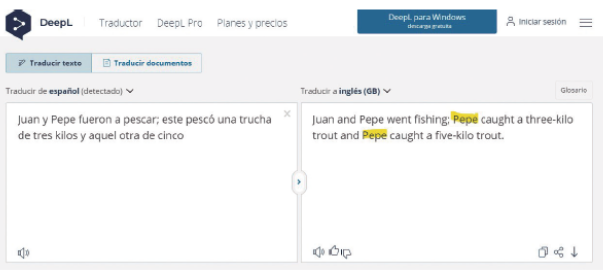
\includegraphics[width=9cm]{error de concordancia.PNG}
        \label{foto}
        \caption{Ejemplo de error de concordancia en el traductor de DeepL}
    \end{figure}
\subsubsection*{3. Uso incorrecto de tiempos verbales}
Los tiempos verbales no son los mismos para todos los idiomas. Así como, mil millones en español son un billón en inglés, los tiempos verbales equivalentes tienen diferentes nombres entre cada idioma.

Por ejemplo, el presente continuo en inglés equivale al presente indicativo en español, se debe tener cuidado con esto, porque frases en inglés como “I am not feeling well” se interpreta de manera literal al español como “No me estoy sintiendo bien”. Si bien, el mensaje se entiende, una manera más natural de decir esta frase es “No me siento bien” o “No me encuentro bien”.

 \textbf{c) Errores semánticos}
 
 Este error sucede cuando el traductor automático no comprende la naturaleza del texto y hace traducciones sin sentido. Se puede encontrar estos errores en temas especializados, como medicina, psicología o alguna ingeniería, en el que las palabras comunes no tienen su significado común.
 
 Este es el caso de la oración en inglés “respiratory compromise” que el traductor lo interpreta como “compromiso respiratorio”, una oración sin sentido, la traducción correcta es “insuficiencia cardiaca”, que se refiere a una condición médica.
 
  \textbf{d) Errores orto-tipográficos}
  \subsubsection*{1. Alteración de la puntuación}

  Los idiomas tienen reglas de ortográficas que son diferentes entre cada una de ellas, un ejemplo conocido es que en inglés no se usa la tilde para mostrar la entonación más fuerte, mientras que en español sí. La tilde no suele ser un problema para la traducción automática, pero no podemos decir lo mismo de otras reglas formales que se utilizan, que si bien no suelen afectar el mensaje, si deja en evidencia, requiere intervenciones para las correcciones.
  
  En la Figura 6 se puede observar cómo se traduce una carta formal del inglés al español, también se puede observar que después del saludo el traductor no cambia la coma por los dos puntos, que son los que se utilizan en cartas y correos formales.

  \begin{figure}[htp]
        \centering
        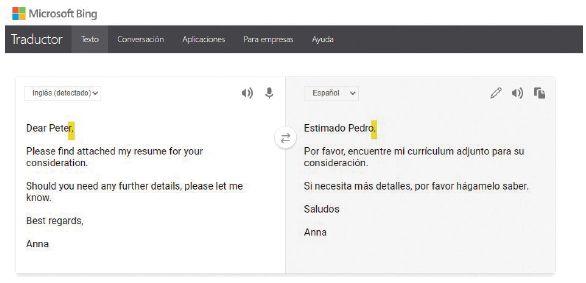
\includegraphics[width=9cm]{alteracion de puntuacion.PNG}
        \label{foto}
        \caption{Ejemplo de alteración de la puntuación al utilizar Bing Microsoft Translator}
    \end{figure}

\subsubsection*{2. Uso incorrecto de mayúsculas y minúsculas}
El uso de las mayúsculas y las minúsculas es, como todo lo anterior, diferente entre cada idioma. En las traducciones no suele adecuarse el uso de estas a su idioma de destino. Este problema se suele encontrar en los títulos, en inglés se escriben todas las palabras de un título en mayúscula, exceptuando las preposiciones, pero en español esta regla no se cumple, aun así, el traductor no aplica las reglas.




\section{Conclusión}
Machine translation a lo largo de los años ha sido una gran ayuda para el ser humano a la hora de comunicarse con otras personas. Estos traductores no son perfectos y muchos de ellos tienen errores lingüísticos que no pueden ser resueltos satisfactoriamente por computadoras, ya que son incapaces de pensar como seres humanos. Por lo que en algunos casos se requiere la intervención humana, pero a pesar de esto se ejemplifica que la traducción automática reemplazaría a los traductores humanos y ya no sería su aporte necesario.

La traducción automática es de gran ayuda para el aprendizaje y así poder tener el conocimiento de otros pensadores que no hablan nuestra misma lengua. A pesar de que la tecnología ha avanzado mucho, los sistemas que se utilizan para la traducción contienen errores, por lo que todavía los traductores no nos ofrecen una ayuda al cien por ciento, pero nos agilizan una gran parte, principalmente en áreas de estudio y en empresas con temas de trabajo.

Existen diferentes tipos de Machine Translation que se definieron anteriormente, cada uno de estos traductores utilizan diferentes algoritmos y programas muy avanzados para que logren su función, y a pesar de que nos dan una traducción al instante lleva un trabajo complejo, pero de igual manera siguen existiendo errores.

De los tipos de traductores podemos observar que el tipo neuronal es el más adecuado, ya que es el más nuevo en cuanto a traducción automática y en él podemos tener la combinación de una inteligencia artificial y la experiencia del traductor humano, por lo que al trabajar en conjunto podemos tener un porcentaje de error menor y esto va a hacer que el sistema vaya aprendiendo en cuanto al traductor humano le vaya corrigiendo y el software va a aprender gracias a esa inteligencia artificial.


\begin{thebibliography}{00}
\bibitem{b1}Arnold, D. Balkan, L. Meijer, S. Humphreys, R.L. Sadler Louisa. (1994). Machine Translation: An Introductory Guide. NCC Blackwell.

\bibitem{b2} Borges, Y., & Mercant, F. (2019). Herramientas para traducción automática Guaraní-Español.
\url{https://www.colibri.udelar.edu.uy/jspui/bitstream/20.500.12008/24378/1
/BM20.pdf  Borges, Y., & Mercant, F. (2019). Herramientas 
para traducción automática Guaraní-Español.}

\bibitem{b3}E.F.K.Koerner, y  R.E.Asher. (1995). Machine Traslation: A brief history. En W.John. Hutchins. (Ed.), Concise history of the language sciences: from the Sumerians to the cognitivists (pp. 431 - 445). Oxford: Pergamon Press.

\bibitem{b4}Etchegoyhen, T., Arzelus, H., Gete, H., Álvarez, A., Hernaez, I., Navas, E., González-Docasal, A., Osácar, J., Benites, E., Ellakuria, I., Calonge, E., & Martin, M. (2020). MINTZAI: Sistemas de Aprendizaje Profundo E2E para Traducción Automática del Habla. Procesamiento Del Lenguaje Natural, 65, 97-100. https://www.proquest.com/scholarly-journals/mintzai-sistemas-de-aprendizaje-profundo-e2e-para/docview/2768727022/se-2


\bibitem{b5} Grace Hui-chin Lin, y Paul Shih Chieh Chien. (2009). Machine Translation for Academic Purposes. En Grace Hui-chin Lin, y Paul Shih Chieh Chien. (Ed.), Proceedings of the International Conference on TESOL and Translation (pp. 133 - 148). 

\bibitem{b6}Houghton, J. (3 de marzo 2020). Lost in Machine Translation: una pequeña introducción a la MT. Ideas Worth Translating. 
\url{https://www.ibidemgroup.com/edu/introduccion-machine-translation-mt/}

\bibitem{b7}Kenny, D (ed.). (2022). Machine translation for everyone: Empowering users in the age of artificial intelligence (Translation and Multilingual Natural Language Processing 18). Berlin: Language Science Press. \url{https://langsci-press.org/catalog/book/342}

\bibitem{b8}Le Scao, T. (14 de mayo 2020). A brief history of Machine Translation paradigms. Ideas Worth Translating. https://www.ibidemgroup.com/edu/breve-historia-traduccion-automatica/

\bibitem{b9}Maldonado González, M. C., Liébana González, M. (2021). Los motores de traducción automática y su uso como herramienta lexicográfica en la traducción de unidades léxicas aisladas. Círculo de Lingüística Aplicada a la Comunicación, 189-212.

\bibitem{b10} mochooss. (2015, septiembre 24). La traducción automática basada en reglas (RBMT). mochooss. https://mochooss.wordpress.com/2015/09/24/la-traduccion-automatica-basada-en-reglas-rbmt/

\bibitem{b11}Montero Languaje Services. (7 de abril de 2022). Obtenido de https://montero-ls.com/aplicaciones-de-la-traduccion-automatica/#

\bibitem{b12} Poibeau, T. (2017). Machine Traslation. Massachusetts Institute of Technology. 

\bibitem{b13}Pym, A., & Torres-Simón, E. (2021). Efectos de la automatización en las competencias básicas del traductor: la traducción automática neuronal. Ocupaciones y lenguaje. Indicadores y análisis de competencias lingüísticas en el ámbito laboral, 479-509.

\bibitem{b14}Traducción Automática Basada en Estadísticas. (2016, septiembre 20). traddraft. https://traddraft.wordpress.com/2016/09/20/traduccion-automatica-basada-en-estadisticas/ 

\bibitem{b15}Trujillos, L. (2020). Aproximación al uso de la traducción automática con posedicion en el ámbito de la traducción medica: opinión de traductores médicos profesionales [Trabajo Final de Máster Investigador].

\bibitem{b16}Wang, H. Wu, H. He, Z. Huang, L. Ward, C, K (2022). Progress in Machine Translation. Engineering, Volumen 18, pp. 143 - 153. https://www.sciencedirect.com/science/article/pii/S2095809921002745

\bibitem{b17}Yuqo, H. (2017, septiembre 29). Nacimiento e historia de la traducción automática. Yuqo. https://www.yuqo.es/nacimiento-e-historia-de-la-traduccion-automatica/



\end{thebibliography}




%% that's all folks
\end{document}


